\section{Giới thiệu}

Zero-shot learning (ZSL) \cite{28, 37, 58} là một mô hình học tập cơ bản trong thị giác máy tính cho phép các mô hình nhận dạng các lớp chưa từng thấy trong quá trình huấn luyện. Các phương pháp ZSL thường chuyển đổi việc phân loại thành một nhiệm vụ hồi quy, trong đó các bộ mô tả ngữ nghĩa cấp lớp, chẳng hạn như các thuộc tính \cite{21} đóng vai trò là các nhãn mềm. Ví dụ, mỗi chiều của một véc-tơ thuộc tính có thể chỉ ra sự hiện diện hoặc vắng mặt của một khái niệm như màu hồng. Tại thời điểm kiểm tra, véc-tơ thuộc tính được dự đoán sẽ được so sánh với các thuộc tính của các lớp chưa từng thấy, và lớp tương tự nhất sẽ được chọn.

Sự sai lệch ngữ nghĩa (Semantic misalignment) là một thách thức cơ bản trong ZSL \cite{1, 4, 9, 27, 30, 46}. Hình ảnh thô thường chứa các chi tiết không liên quan đến ngữ nghĩa không được mô tả bởi các thuộc tính. Ví dụ, sự lộn xộn của nền, các biến thể ánh sáng, hoặc các đối tượng xung quanh có thể tạo ra các mẫu gây hiểu lầm. Do đó, mô hình có thể tập trung vào các đặc trưng không quan trọng thay vì các tín hiệu ngữ nghĩa có liên quan. Vì các chi tiết ngoại lai này không được chú thích rõ ràng trong các véc-tơ thuộc tính, chúng phá vỡ sự liên kết thị giác-ngữ nghĩa bằng cách làm loãng các thuộc tính chính như màu sắc và hình dạng. Điều này làm cho mô hình khó nhận dạng các lớp chưa từng thấy hơn.

Như được trình bày trong Hình \ref{fig:approaches}(a), các công trình trước đây đã cố gắng giải quyết vấn đề này bằng cách tinh chỉnh hoặc tách rời các đặc trưng, để thông tin nhất quán về mặt ngữ nghĩa được bảo tồn trong khi thông tin không liên quan đến ngữ nghĩa bị triệt tiêu \cite{1, 9, 27, 30}. Do đó, các đặc trưng thị giác nhất quán về mặt ngữ nghĩa được bảo tồn có thể tăng cường sự liên kết thị giác-ngữ nghĩa. Mặc dù các cải tiến sau xử lý (post hoc) này hữu ích, chúng không thể ngăn chặn hoàn toàn thông tin ngoại lai thấm vào các biểu diễn đã học.

Song song đó, các kiến trúc dựa trên transformer \cite{48} đã nổi lên như những 'backbone' mạnh mẽ trong các nhiệm vụ thị giác \cite{26} bằng cách mô hình hóa hình ảnh dưới dạng chuỗi các bản vá. Dưới ánh sáng của khả
% \newpage
\begin{figure*}[t]
    \centering
    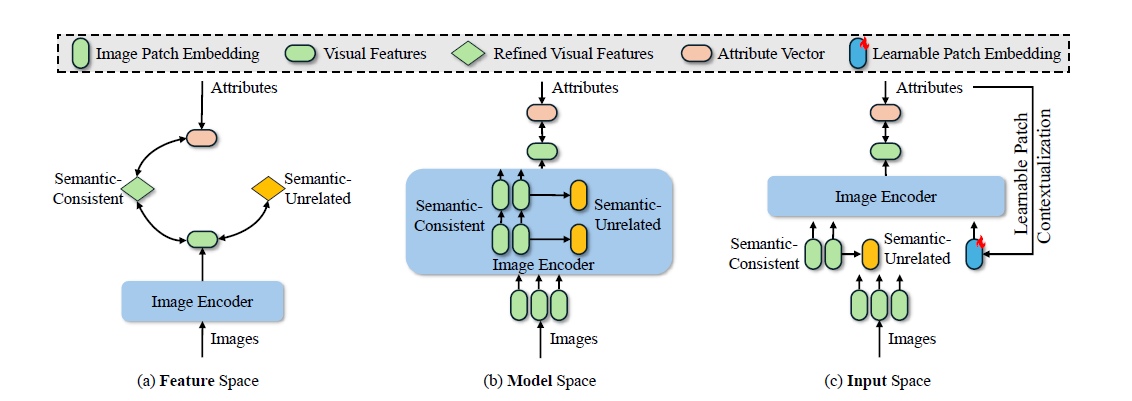
\includegraphics[width=\textwidth]{Image/Figure 1.PNG}
    \caption{Các phương pháp để giảm thiểu sự sai lệch ngữ nghĩa cho ZSL. (a) Các phương pháp tách rời loại bỏ thông tin không liên quan đến ngữ nghĩa trong không gian đặc trưng. (b) Các phương pháp hướng dẫn ngữ nghĩa tiến bộ loại bỏ các bản vá không liên quan đến ngữ nghĩa trong không gian mô hình. (c) SVIP của chúng tôi xác định các bản vá hình ảnh không liên quan đến ngữ nghĩa ở vị trí đầu vào và thay thế chúng bằng các bản vá thị giác được bối cảnh hóa về mặt ngữ nghĩa.}
    \label{fig:approaches}
\end{figure*}

năng học biểu diễn mạnh mẽ của Vision Transformers (ViTs) \cite{19, 66}, các nhà nghiên cứu trong cộng đồng ZSL đang chuyển sang thiết kế các phương pháp dựa trên ViT \cite{4, 17, 32}. Hành vi mô hình hóa bản vá cho phép xác định các bản vá không liên quan đến ngữ nghĩa. Như trong Hình \ref{fig:approaches}(b), ZSLViT \cite{4} loại bỏ dần các token thị giác không ánh xạ tới ngữ nghĩa trong không gian mô hình. Tuy nhiên, nghiên cứu đã chỉ ra rằng các đặc trưng ngữ nghĩa có thể bị loãng ở các lớp sâu hơn của ViT \cite{40}, khiến cho thông tin không liên quan đến ngữ nghĩa dễ dàng tồn tại và có khả năng làm ô nhiễm các đặc trưng thị giác cuối cùng.


Như trên, các phương pháp này hoặc loại bỏ các đặc trưng không liên quan đến ngữ nghĩa sau khi trích xuất các đặc trưng thị giác bị vướng víu, hoặc trong quá trình trích xuất các đặc trưng thị giác, chúng không hoàn toàn ngăn chặn các đặc trưng đó ảnh hưởng đến các biểu diễn đã học. Do đó, một câu hỏi nghiên cứu hấp dẫn được đặt ra: \textbf{Chúng ta có thể loại bỏ hoặc tái sử dụng một cách ưu tiên các bản vá không liên quan đến ngữ nghĩa ở giai đoạn đầu vào để tránh vướng víu chúng vào các đặc trưng đã học không?}

Để đạt được mục tiêu này, chúng tôi đề xuất \textbf{SVIP}, Semantically contextualized VIsual Patch, một framework dựa trên ViT được thiết kế để giảm thiểu thông tin không liên quan đến ngữ nghĩa và tăng cường sự lan truyền ngữ nghĩa-thị giác trong ZSL. Như được trình bày trong Hình \ref{fig:approaches}(c), không giống như các công trình trước đây cắt tỉa hoặc tinh chỉnh các đặc trưng sau khi chúng đã được trích xuất, SVIP xác định và bối cảnh hóa các bản vá này ngay từ đầu.

Cụ thể, để giải quyết vấn đề sai lệch ngữ nghĩa một cách toàn diện, chúng tôi đề xuất cơ chế lựa chọn bản vá tự giám sát nhằm học cách xác định các bản vá không liên quan đến ngữ nghĩa trong không gian đầu vào, tức là, trước khi đưa vào các khối transformer. Đặc biệt, chúng tôi tổng hợp các ma trận trọng số tự chú ý trên tất cả các khối transformer, mang lại sự hiểu biết ngữ nghĩa đáng tin cậy về tầm quan trọng của bản vá trong toàn bộ ViT. Để giảm thiểu tác động tiêu cực của các bản vá không liên quan đến ngữ nghĩa đối với các bản vá liên quan đến ngữ nghĩa, chúng tôi huấn luyện một bộ phân loại bản vá để xác định các bản vá đầu vào không liên quan đến ngữ nghĩa, sử dụng sự giám sát từ ma trận chú ý tổng hợp. Tại thời điểm kiểm tra, bộ phân loại bản vá có thể trực tiếp ngăn chặn các bản vá không liên quan đến ngữ nghĩa lan truyền vào quá trình trích xuất đặc trưng. Một khi các bản vá không liên quan đến ngữ nghĩa được xác định trong chuỗi đầu vào, một giải pháp đơn giản là loại bỏ chúng khỏi chuỗi đầu vào. Tuy nhiên, điều này có thể phá vỡ cấu trúc đối tượng trên hình ảnh. Thay vào đó, chúng tôi đề xuất che các bản vá không liên quan đến ngữ nghĩa bằng một bản vá ngữ cảnh có thể học được. Bản vá ngữ cảnh ngữ nghĩa được khởi tạo bằng các nhúng từ cấp thuộc tính cung cấp thông tin ngữ nghĩa phong phú. Các bản vá đầu vào được bối cảnh hóa này có thể tăng cường tương tác thị giác-ngữ nghĩa trong suốt quá trình trích xuất đặc trưng thị giác. Nhìn chung, những đóng góp của bài báo này là:
\begin{itemize}
    \item Chúng tôi giới thiệu Semantically contextualized VIsual Patch (SVIP), một framework dựa trên ViT để giải quyết vấn đề sai lệch ngữ nghĩa trong zero-shot learning. Nó nhấn mạnh việc xử lý sớm các bản vá không liên quan đến ngữ nghĩa để đạt được một không gian đặc trưng tập trung và rõ ràng hơn cho ZSL.
    \item Chúng tôi đề xuất một chiến lược lựa chọn bản vá tự giám sát để xác định các bản vá không liên quan đến ngữ nghĩa bằng cách sử dụng các điểm chú ý được tổng hợp từ ma trận trọng số tự chú ý trên các khối ViT. Chúng tôi đề xuất bối cảnh hóa ngữ nghĩa bản vá bằng cách đưa các nhúng từ cấp thuộc tính vào các bản vá không liên quan đến ngữ nghĩa, đảm bảo rằng thông tin ngữ nghĩa được tích hợp vào các biểu diễn thị giác từ các lớp ban đầu của transformer.
    \item SVIP đạt được kết quả hiệu suất hiện đại trên ba bộ dữ liệu ZSL tiêu chuẩn trên cả cài đặt ZSL và ZSL tổng quát, chứng tỏ hiệu quả trong việc giảm thiểu sự sai lệch ngữ nghĩa trong không gian đầu vào.
\end{itemize}